\documentclass[conference]{IEEEtran}
\IEEEoverridecommandlockouts
\usepackage{cite}
\usepackage{amsmath,amssymb,amsfonts}
\usepackage{algorithmic}
\usepackage{graphicx}
\usepackage{textcomp}
\usepackage{xcolor}
\usepackage{minted}
\usepackage{enumitem}
\usepackage{hyperref}
\usepackage{float}
\usepackage{tabularx}
\usepackage{floatrow}
\usepackage{algorithm}
\usepackage{algorithmic}
\usepackage{listings}
\usepackage{listings}
\usepackage{color}

\definecolor{codegray}{rgb}{0.5,0.5,0.5}
\definecolor{codeblue}{rgb}{0.25,0.5,0.75}
\definecolor{codepurple}{rgb}{0.58,0,0.82}

\lstdefinestyle{mystyle}{
    backgroundcolor=\color{white},   
    commentstyle=\color{codegray},
    keywordstyle=\color{codeblue},
    numberstyle=\tiny\color{codegray},
    stringstyle=\color{codepurple},
    basicstyle=\ttfamily\footnotesize,
    breakatwhitespace=false,         
    breaklines=true,                 
    captionpos=b,                    
    keepspaces=true,                 
    numbers=left,                    
    numbersep=5pt,                  
    showspaces=false,                
    showstringspaces=false,
    showtabs=false,                  
    tabsize=2
}

\lstset{style=mystyle}

\newcommand{\MYhref}[3][blue]{\href{#2}{\color{#1}{#3}}}

\hypersetup{
    colorlinks=true,
    linkcolor=blue,
    filecolor=magenta,      
    urlcolor=cyan,
    pdftitle={Overleaf Example},
    pdfpagemode=FullScreen,
    }
\urlstyle{same}
\def\BibTeX{{\rm B\kern-.05em{\sc i\kern-.025em b}\kern-.08em
    T\kern-.1667em\lower.7ex\hbox{E}\kern-.125emX}}
\begin{document}

\title{Visual Recognition : Final Assignment\\
{\footnotesize \textsuperscript{}}
\thanks{}
}


\author{\IEEEauthorblockN{Subhajeet Lahiri}
\IEEEauthorblockA{\textit{IMT2021022} \\
\textit{}\\
 \\
}
\and
\IEEEauthorblockN{Sai Madhavan G}
\IEEEauthorblockA{\textit{IMT2021101} \\
\textit{}\\
 \\
}
\and
\IEEEauthorblockN{Aditya Garg}
\IEEEauthorblockA{\textit{IMT2021545} \\
\textit{}\\
 \\
}

}

\maketitle

\begin{abstract}
In this report, we delve into Visual Question Answering (VQA) using various image and text encoders. Specifically, we explore the performance of DINO and ResNet-50 as image encoders, coupled with BERT as the text encoder, integrating them through a co-attention mechanism. Our investigation extends to fine-tuning these models and experimenting with the depth and architecture of the co-attention block we implemented. Additionally, we explore the efficacy of Lora fine-tuning in enhancing model performance. Our findings offer valuable insights into the interplay between different encoder architectures and co-attention mechanisms.
\end{abstract}


\begin{center}
Link to the \MYhref{https://github.com/Gapes21/VisualQuestionAnswering}{GitHub Repository}.\\
Link to the \MYhref{https://github.com/Gapes21/VisualQuestionAnswering}{Model Snapshots}.
\end{center}

%___________________________________________________________________________________________________________________________________

\vspace{0.5cm} \hrule{} \vspace{0.5cm}
\section*{\textbf{A) Sampling and Dataset creation}}
\label{sampling}

For this project, we utilized the Visual Question Answering (VQA) Dataset released by Georgia Tech, specifically focusing on the Balanced Real Images subset. Given the large size of the dataset, we were instructed to use only 25\% of the training images to make the task more manageable. 

\subsection*{Random Sampling}
To achieve the 25\% subset, we employed a random sampling method. This approach involves selecting images at random from the dataset, ensuring each image has an equal chance of being included. The code snippet below demonstrates our sampling process:

\begin{lstlisting}[language=Python]
def createRandomSample(p : float):
    sample = set()
    imgfiles = os.listdir('./../RawImages/images/')[1:]
    for img in imgfiles:
        if np.random.choice([0, 1], p = [1 - p, p]):
            sample.add(FiletoId(img))
    return sample
sample = createRandomSample(0.25)
\end{lstlisting}

This method was chosen due to its simplicity and effectiveness. Random sampling ensures that the subset is representative of the entire dataset, capturing a diverse range of images and questions without introducing any bias. This randomness is crucial in avoiding overfitting and ensuring that the model generalizes well to unseen data.

By leveraging this approach, we maintain the integrity and diversity of the original dataset, facilitating robust training and evaluation of our VQA model.

\subsection*{Hugging face dataset}

To facilitate easy access and management of our sampled dataset, we created a Hugging Face dataset. This approach allows us to leverage the powerful data handling and machine learning tools provided by the Hugging Face ecosystem, streamlining the data pre-processing phase and enhancing our model training and evaluation process.
The final dataset is structured to contain pairs of questions and images as input, with the corresponding answers as labels. Each entry in the dataset includes:
\begin{itemize}
    \item \textbf{Image}: The image file associated with the question.
    \item \textbf{Question}: The text of the question related to the image.
    \item \textbf{Answer}: The textual answer to the question.
\end{itemize}

We have the following observations about the data : 
\begin{itemize}
    \item The answer text is generally very short and there are 9214 distinct answers in the sampled dataset with around 110k samples. This, coupled with the required reporting metric being accuracy and f1 score leads us to training a classifier on the answer space.
    \item Within the dataset, there are some super classes such as 'yes' and 'no', which constitute almost half of the labels.
    The figure below demonstrates the stated fact : 
    \begin{figure}[H]
        \centering
        \includegraphics[width=0.87\linewidth]{sampling_section/image.png}
    \end{figure}
\end{itemize}

%___________________________________________________________________________________________________________________________________

\vspace{0.5cm} \hrule{} \vspace{0.5cm}
\section*{\textbf{B) Base Model - DINO + Bert with a single co-attention layer}}
\label{basemodel}

%___________________________________________________________________________________________________________________________________

\vspace{0.5cm} \hrule{} \vspace{0.5cm}
\section*{\textbf{C) Base Model - DINO + Bert with a single co-attention layer}}
\label{basemodel}

\begin{figure*}
    \centering
    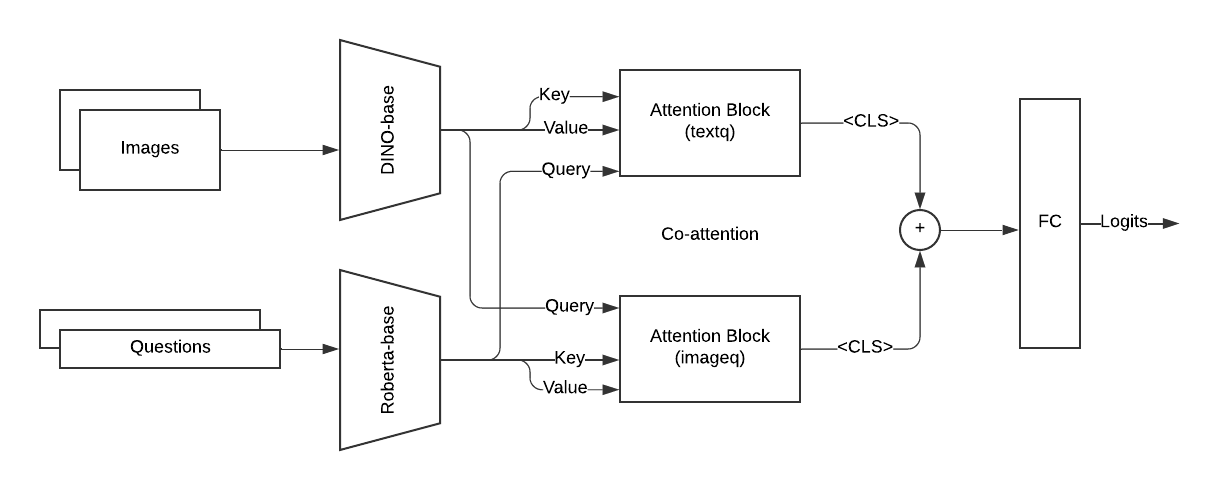
\includegraphics[width=1\linewidth]{dinobert/dinobert_base.png}
    \caption{Dinobert base model architecture}
    \label{dinobert_base}
\end{figure*}

For our initial experiments, we employed a base model consisting of a pre-trained image encoder and a pre-trained text encoder. Specifically, we used \textbf{facebook/dinov2-base} for the image encoder and \textbf{FacebookAI/roberta-base} for the text encoder. 
The model architecture is demonstrated by Fig. \ref{dinobert_base}.

\subsection*{Encoders}

The `facebook/dinov2-base` model is based on the Vision Transformer (ViT) architecture, which processes images by dividing them into patches and using transformer layers to capture spatial relationships and features. The `FacebookAI/roberta-base` model is a variant of the BERT architecture designed for robust text understanding, which uses transformer layers to capture the contextual relationships between words in a sentence.

\subsection*{Combining Encoder Outputs}

To combine the outputs of these models, we implemented a co-attention mechanism using `nn.MultiheadedAttention` with a single attention head. This allows the model to focus on relevant parts of both the image and the text simultaneously. The process is as follows:

\begin{itemize}
    \item We extract (Sequence length, Embedding dimension) shaped vectors from both the text and the image encoders. The sequence length for the image encoder is 257 (An image is worth 16 * 16 words) and that of the text encoder depends on the length of the question and is typically around 8 - 10. The embedding dimension is 768 for both the encoders.
    \item We apply co-attention between the image and the text encoders. Specifically, values and keys from the text encoder are used to answer queries from the image encoder and vice-versa.
    \item We combine the two co-attention outputs by extracting the attended [CLS] token vectors, and then adding them to get a single [CLS] token vector of dimension (batch\_size, 768). It now contains information from both the image and the text.
    \item We pass this vector through a fully connected (FC) layer to obtain a 9214-dimensional vector representing the logits.
\end{itemize}

\subsection*{Training and Performance}
The model was trained using cross-entropy loss. Despite/due to the unsophisticated architecture, the base model achieved an accuracy of 18.61\%. The performance metrics are summarized in the table below:

\begin{table}[H]
    \centering
    \begin{tabular}{|c|c|}
        \hline
        \textbf{Metrics} & \textbf{Values} \\
        \hline
        Accuracy (Validation) & 18.61\% \\
        Accuracy (Training) & 19.33\% \\
        Precision (Validation) & 0.07 \\
        Recall (Validation) & 0.19 \\
        f1-score (Validation) & 0.09 \\
        Time taken per epoch & 1 hr 07 min \\
        Total time taken & 5 hr 33 min\\ 
        \hline
    \end{tabular}
    \vspace{1mm}
    \caption{Performance metrics of the base model}
\end{table}
A significant issue observed was that the model predominantly predicted only 4 classes: "yes", "no", "snowboarding" and "skiing" - two of them being one of "super" classes pointed out above.
\begin{table}[H]
    \centering
    \begin{tabular}{|c|c|}
        \hline
        \textbf{Label} & \textbf{Predictions} \\
        \hline
        Yes & 1548 \\
        No & 7755 \\
        Snowboarding & 178\\
        Skiing & 4\\
        \hline
    \end{tabular}
    \vspace{1mm}
    \caption{Distribution of predictions for different classes}
\end{table}

%___________________________________________________________________________________________________________________________________

\vspace{0.5cm} \hrule{} \vspace{0.5cm}
\section*{\textbf{D) Model Optimization 1: Lighter model without co-attention}}
\label{smallermodel}
\begin{figure*}
    \centering
    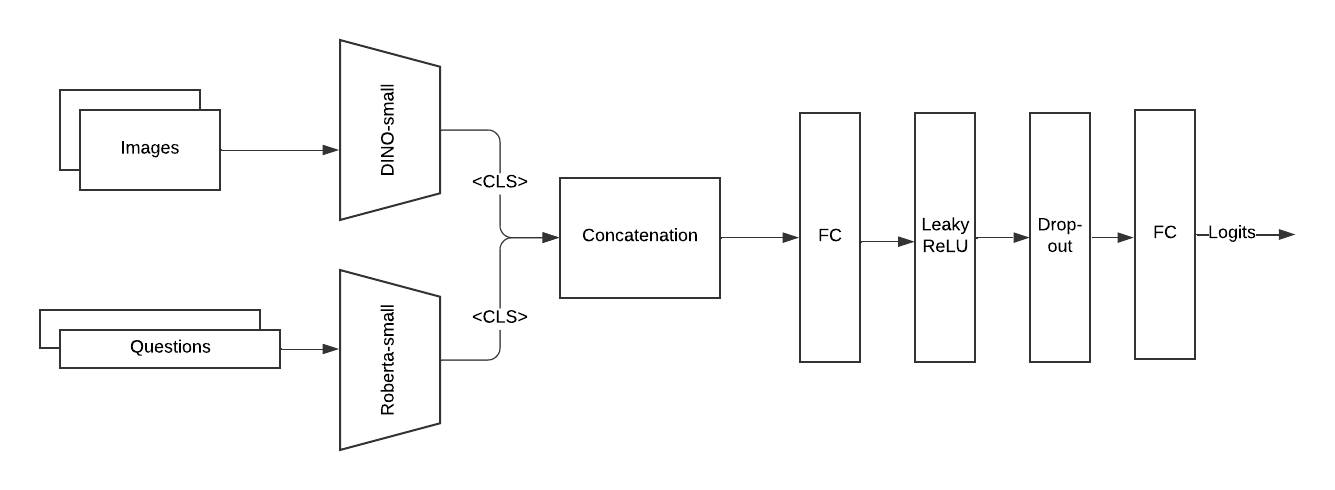
\includegraphics[width=1\linewidth]{dinobert/dinobert_small.png}
    \caption{Dinobert small variant architecture}
    \label{dinobert_small}
\end{figure*}

In an effort to address the disparity between the number of samples and the model size, we introduced two optimizations to our model. The model architecture is demonstrated in Fig. \ref{dinobert_small}.

\subsection*{Model Size Reduction}
Firstly, we down-scaled the pre-trained encoders from their base variants to their smaller counterparts. Specifically, we replaced the original models with `smallbenchnlp/roberta-small` for BERT and `facebook/dinov2-small` for ViT. The rationale behind this step is that the original models had over 400 million parameters, whereas our dataset consisted of only 100k samples. By reducing the model size to 135 million parameters, we aimed to better match the model complexity with the available data.

\subsection*{Removal of Co-Attention Mechanism}

Secondly, we experimented with removing the co-attention mechanism and instead opted for a simpler approach of concatenating the output of the encoders and passing them through fully connected (FC) layers directly. This decision was based on the hypothesis that the complexity introduced by the co-attention mechanism may not be necessary for our task, and a simpler architecture could suffice.

\subsection*{Training Details and Performance}

We trained the optimized model for 10 epochs with an initial learning rate of 5e-4. We decayed the learning rate by a factor of 0.2 every 2 epochs. The decrease in model complexity led to a significant reduction in training time per epoch, from 1 hour and 10 minutes to 27 minutes.

The resulting model exhibited the following metrics:

\begin{table}[H]
    \centering
    \begin{tabular}{|c|c|}
        \hline
        \textbf{Metrics} & \textbf{Values} \\
        \hline
        Accuracy (Validation) & 19.14\% \\
        Accuracy (Training) & 21.85\% \\
        Precision (Validation) & 0.07 \\
        Recall (Validation) & 0.19 \\
        f1-score (Validation) & 0.10 \\
        Time taken per epoch & 27min \\
        Total time taken & 4 hr 31 min \\ 
        \hline
    \end{tabular}
    \vspace{1mm}
    \caption{Performance metrics of the optimized model}
\end{table}

\subsection*{Observations}
\begin{itemize}
    \item Despite the optimizations, the model did not achieve a significant improvement in accuracy. This can largely be attributed to the model's increasing bias towards the "super" classes ("yes" and "no") as training progressed. Initially, the untrained model exhibited predictions across over 1,000 classes on the validation data. However, towards the end of training, it predominantly focused on predicting the "yes" and the "no" classes.
    \item Accuracy scores of around 21\% can be obtained if the model just learns that "yes" is the most frequent class and predicts it for every sample.
\end{itemize}


\begin{table}[H]
    \centering
    \begin{tabular}{|c|c|}
        \hline
        \textbf{Label} & \textbf{Predictions} \\
        \hline
        Yes & 6714 \\
        No & 2771 \\
        \hline
    \end{tabular}
    \vspace{1mm}
    \caption{Distribution of predictions for "yes" and "no" classes}
\end{table}

%___________________________________________________________________________________________________________________________________

\vspace{0.5cm} \hrule{} \vspace{0.5cm}
\section*{\textbf{E) Model Optimization 2: Broader model with skip connections}}
\label{dinobertadv}

\begin{figure*}
    \centering
    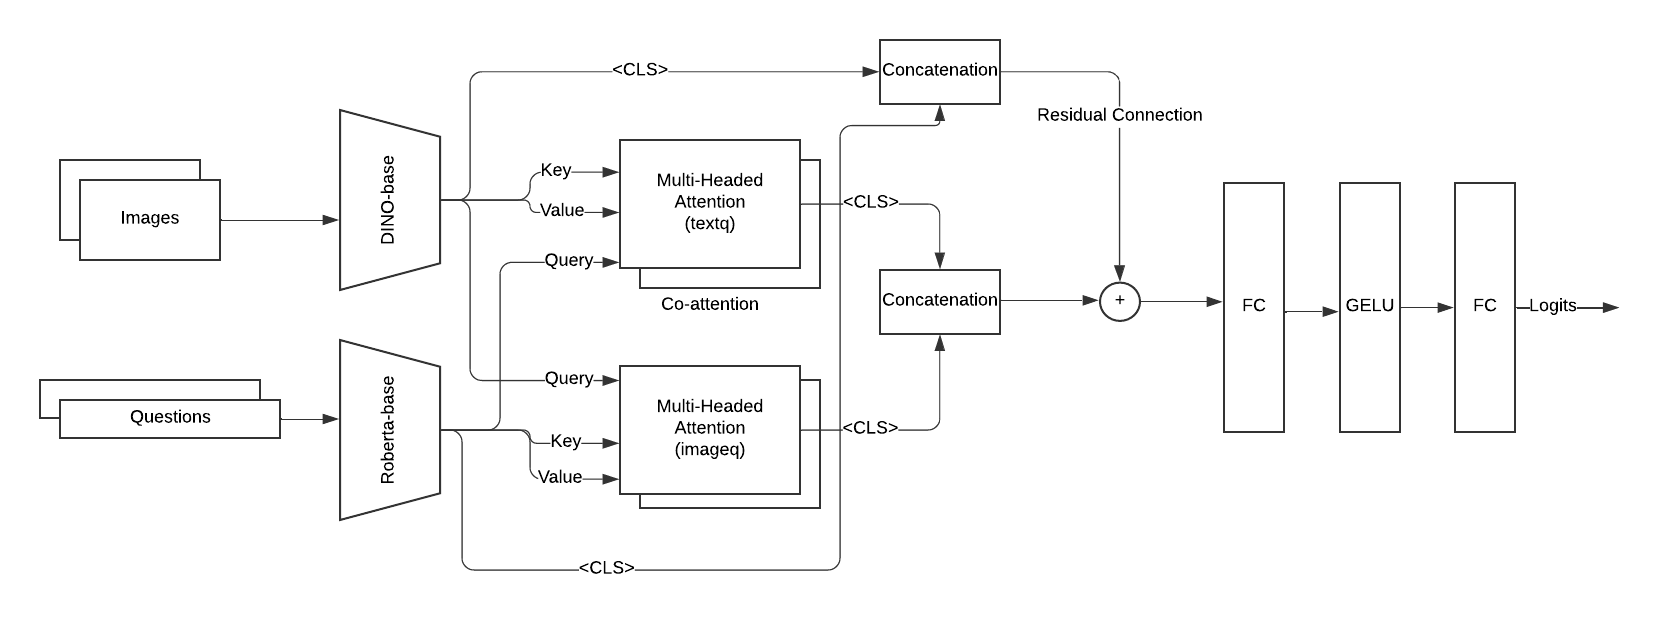
\includegraphics[width=1\linewidth]{dinobert/dinobert_adv.png}
    \caption{Dinobert advanced variant architecture}
    \label{dinobert_adv}
\end{figure*}

\begin{figure}
    \centering
    \includegraphics[width=0.75\linewidth]{dinobert/acclosscurve.png}
    \caption{Accuracy, loss curve - X-axis: epochs, Y-axis: the blue line denotes percentage accuracy while the yellow line denotes loss}
\end{figure}

\vspace{0.5cm} \hrule{} \vspace{0.5cm}
\section*{\textbf{F) Conclusion}}
\label{conclusion}


%_________________________________________________________________________________________________________________________________________________
\

\vspace{0.5cm} \hrule{} \vspace{0.5cm}
\begin{thebibliography}{00}
\bibitem{b1} https://www.analyticsvidhya.com/blog/2019/10/detailed-guide-powerful-sift-technique-image-matching-python/
\end{thebibliography}
\vspace{12pt}

\end{document}
